\documentclass{article}
\usepackage[utf8]{inputenc}
\usepackage[a4paper,margin=2.5cm]{geometry}

\title{Perspectives in Mathematics - History of Statistics}
\author{Stefan Eng}
\date{December 2018}

\usepackage{natbib}
\usepackage{graphicx}
\usepackage{url}
\usepackage{amsmath}
\usepackage{setspace}
\usepackage{booktabs}

\onehalfspacing

\begin{document}

\maketitle

\section{Introduction}
This short essay is a brief overview of modern statistics during the period from late 1800s to about 1940s.
It describes briefly Karl Pearson, Sir Francis Galton, William Sealy Gosset, and of course Ronald Fisher.
It is difficult to condense this period of time into a short essay but some major accomplishments are described such as Pearson's contribution to probability distributions, Gosset's ``Student's t-test'' and distribution, Fisher's work on experimental design and the analysis of variance.
The people selected were some of the most influential people in statistics and the connection between them was fascinating.
The rivalry between Pearson ``the communist'' and Fisher ``the fascist'' reads like it should be a movie script.
These men made a large impact on the world of statistics.
Their influence extended well beyond statistics into other fields.
Most cases they had a positive impact but a notable exception such as eugenics, the "set of beliefs and practices that aims at improving the genetic quality of a human population." \cite{wiki:eugenics}.
This led to the ``science'' that influenced Hilter and the Nazis.
While this is in no way a comprehensive list of the history of statistics, the people described in this essay had an enormous influence on mathematics, statistics, and science in general \cite{wiki:history_stats}.

\subsection{Sir Francis Galton (1822 - 1911)}
Francis Galton, lived from 1822 to 1911 was Karl Pearson's advisor.
Galton was the first to propose using fingerprints in crime scene investigation.
He was knighted in 1909 thus gaining the title of ``sir'' \cite{britannica_galton}.
Galton's cousin was the famous scientist Charles Darwin whose book ``On the Origin of Species'' had great influence on him.
Galton [mis]used much of what Darwin wrote, which led to him creating the field of Eugenics which studied how good genetic could be passed down to improve the population.
The idea was that by selectively breeding the population could be used to create better mental and physical characteristics of the population as a whole \cite{britannica_galton}.
Most of Galton's work was involved in Eugenics and one of his more famous experiments is described below.

\subsection{Regression Towards Mediocrity}
In 1886 he published his groundbreaking paper titled ``Regression Towards Mediocrity in Hereditary Stature.'' \cite{galton_regression}.
It was in this paper that he described the phenomenon of ``Regression towards mediocrity'', which is now called ``Regression to the mean''.
Galton noticed this in his biometrical laboratory where he measured the heights of parents and children in London.
The parents that were extremely tall tended to have children which were shorter than them.
Similarly, the children tended to be taller than their parents when their parents were unusually short.

According to the Cambridge dictionary of statistics, the modern definition of Regression to the mean is ``...now generally used to label the phenomenon that a variable that is extreme on its first measurement will tend to be closer to the centre of the distribution for a later measurement.'' \cite{cambridgestats}

Using modern notation the situation Galton described was as follows.
We can represent the height of parent $i$ as the variable, $x_i$, and height of child of parents $i$ as the dependent variable, $y_i$.
Then we can express Galton's experiment using simple linear regression
$$
y_i = \beta_0 + \beta_1 x_i + \epsilon_i
$$
We assume that the $\epsilon_i$ are independent random variables that have constant variance $Var(\epsilon_i) = \sigma^2$ and centered around 0, $E(\epsilon_i) = 0$.
Minimizing $\epsilon_i = y_i - (\beta_0 + \beta_1 x_i)$ gives us estimates for $\beta_0$ and $\beta_1$ which we write as $\hat{\beta_0}$ and $\hat{\beta_1}$ respectively.
After simplifying the terms we can express them as follows.

\begin{align*}
\hat{\beta_0} &= \overline{y} - \hat{\beta_1} \overline{x}\\
\hat{\beta_1} &= \frac{Cov(X,Y)}{Var(X)}
\end{align*}
Where we define the (uncorrected) variance and covariance as
\begin{align*}
Var(X) &= \frac{1}{n} \sum_{i = 1}^{n} (x_i - \overline{x})^2\\
Var(Y) &= \frac{1}{n} \sum_{i = 1}^{n} (y_i - \overline{y})^2\\
Cov(X,Y) &= \frac{1}{n} \sum_{i = 1}^{n} (x_i - \overline{x})(y_i - \overline{y})\\
\end{align*}
The correlation coefficient is defined then as
$$
r = \frac{Cov(X,Y)}{\sqrt{Var(X) Var(Y)}}
$$
Which means that we can then express $\hat{\beta_1}$ as 
$$
\hat{\beta_1} = r \frac{\sqrt{Var(Y)}}{\sqrt{Var(X)}} 
$$
It follows that
\begin{align*}
    \hat{y} &= \hat{\beta_0} + \hat{\beta_1} x\\
    \hat{y} &=  \overline{y} - \hat{\beta_1} \overline{x} +  \hat{\beta_1} x\\
    \hat{y} - \overline{y} &= \hat{\beta_1} (x - \overline{x})\\
    \hat{y} - \overline{y} &= r \frac{\sqrt{Var(Y)}}{\sqrt{Var(X)}} (x - \overline{x})\\
    \frac{
        \hat{y} - \overline{y}
    } {
    \sqrt{Var(Y)}
    } &=
    r \frac{
        x - \overline{x}
    } {
    \sqrt{Var(X)}
    } 
\end{align*}
What does this tell us about the regression to the mean effect?
Let's assume that there is a positive correlation between the variables $x$ and $y$.
That means that $r > 0$.
Now take our $x$ to be 1 standard deviation greater than the mean.
Thus, $x - \overline{x} = \sqrt{Var(X)}$.
Then
$$
\frac{
        \hat{y} - \overline{y}
    } {
    \sqrt{Var(Y)}
    }
    = r
$$
Tells us that the estimate of $y$ will be $r$ standard deviations bigger than its mean.
Since $r \leq 1$, this will deviate less than the predictor did.
\cite{rice_2007}.
From this equation we also get the interpretation that if we standardize (subtract the mean and divide by the standard deviation) the variables, then the regression coefficient is the slope of the regression line.

\subsection{Karl Pearson (1857 - 1936)}
Karl Pearson was born March 27, 1857 and died on April 27 1936. \cite{wiki:pearson}.
% He was originally born Carl Pearson but changed the spelling of his name to Karl after becoming a strong supporter of Karl Marx.
Pearson became a strong supporter of Karl Marx after studying political science in Germany.
He actually changed the spelling of his name to due to his admiration for Karl Marx \cite{salsburg_2002}.
After returning to England he was more interested in science and mathematics than political science.
He 1892 published ``The Grammar of Science'', which described experimentation and physics in general. This book apparently had an influence on Einstein \cite{wiki:grammar_science}.
Pearson founded a biometric laboratory at University College which he used to collect and analyze biological data. \cite{britannica_pearson}.
He was the founder of the journal \textit{Biometrika} which is still a major journal today.

His many contributions to statistics include: The correlation coefficient, Method of moments, Chi Distance, p-values, Pearson's chi-squared test, Principal component analysis.
In 1900 Pearson created the Chi-Squared test \cite{orig_pearson_chi}.
It is used to test categorical data to see if there is a difference between the different sets of data \cite{wiki:chi_squared}.

\subsection{Probability Distributions}
%% These seem conflicting with wikipedia 
% 
% The first description of a probability distribution date back to Laplace in 1820.
Laplace referred to the distribution of differences between the observed and predicted values as the error distribution, now called the \textit{Laplace distribution} \cite{wiki:laplace_dist}
$$
f(x\mid \mu ,b)={\frac  {1}{2b}}\exp \left(-{\frac  {|x-\mu |}{b}}\right)\,\!
$$
Pearson was the first to use probability distributions to describe the uncertainty in the measurement rather than uncertainty in the errors of the measurement \cite{salsburg_2002}.
Previously deviations from mathematical formulas were thought to be due to the difficulties in measuring rather than an underlying uncertainty.
Pearson went again this method of thinking by claiming that probability distributions are the real object to be studied.
The results of each experiment are just a realization of the probability distribution.
The \textit{parameters}, or unobservable variables in the probability distributions, are what is to be estimated.
This was a huge change in thinking from that there was some correct value or formula that was intrinsically correct.

\subsection{William Sealy Gosset (1876 - 1937)}
He worked for Guinness Beer as a chemist and mathematician.
During this time he was responsible for taking measurements of yeast among other things.
It was during this yeast samples that he realized that the samples followed a Poisson distribution. \cite{salsburg_2002}
He wanted to publish these results since there had not been a practical use for the Poisson distribution.
Guinness beer forbid its employees from publishing articles so Gosset published under the pseudonym ``Student''.
Most of Gosset's work was done under the pseudonym.
In 1908 Gosset published his work which is known as the ``Student's T Test''.
He was interested in smaller data problems, where there were only 10 to 20 measurements.
Previously Pearson's work had been done on thousands of data points.
Gosset's results showed the following: Assume we have $n$ data points, $x_1,\ldots, x_n$ that are independent from a normal distribution mean $\mu$ and variance $\sigma^2$. Let 
$$
\overline{X} = \frac{1}{n} \sum_{i = 1}^n x_i
$$
be the sample mean
and
$$
S^2 = \frac{1}{n-1} \sum_{i = 1}^n(x_i - \overline{x})^2
$$
Then
$$
\frac{\overline{X} - \mu}{S/\sqrt{n}}
$$
Follows a t-distribution with $n-1$ degrees of freedom which is defined as follow
$$
f(t) = \frac{\Gamma[(n + 1) / 2]}{\Gamma(n / 2) \sqrt{n\pi}} \left( 1 + \frac{t^2}{n} \right)^{-(n + 1) / 2}
$$
The t-distribution converges to normal distribution with mean 0 and variance 1 as $n$ goes to infinity.

\subsection{Ronald Fisher (1890 - 1962)}
Ronald Fisher was born in London, February 17, 1890 and died in 1962. \cite{britannica_fisher}
He had major eye problems growing up so his doctor forbid him to read under artificial light. \cite{salsburg_2002}
This led to his tutor talking through and visualizing problems instead of writing them down.
The effects of this can be seen in his later work which showed a great geometric insight of mathematics.

Fisher became interested in eugenics, which is defined as, ``the practice or advocacy of controlled selective breeding of human populations (as by sterilization) to improve the population's genetic composition'' \cite{wiki:eugenics}.
The term was invented by Francis Galton who was previously described.
Fisher's interest in eugenics led him to focus much of his research on genetics.

Fisher worked in agriculture when he made many of his great statistics contributions.
He worked for the Rothamsted Agricultural Experimental Station, in Harpenden, England, from 1919 to 1933.
Fisher had access to 90 years of agricultural data which at the time was useless to the agricultural scientists.
Data was recorded on the size of the harvest along with rain amounts and the fertilizer used for the crop.
All of these data points were used to create a ``fertility index'' which was used to correct the experiments for the conditions such as weather, rainfall, etc.
Fisher found that all of the competing fertility indices across various agricultural stations were essentially the same formulas that were not correctly adjusting for the various conditions of the crops.
It was after working with the agricultural data for a few years that Fisher started the field of experimental design.
He noticed that the data collected was not able to answer the questions about the fertilizer effectiveness.
From this he determined that to perform an experiment first a mathematical model should be created to describe the connection between the data and the outcome being estimated.
This was described in great detail in his book, The Design of Experiments \cite{fisher:1935}, which was published in 1935.

Some of his many other contributions include: Fisher's Exact test, Fisher's principle, Fisher information, Analysis of Variance, Fisher's z-distribution, proved Student's t-statistic, distribution of correlation coefficient, and maximum likelihood estimation \cite{wiki:fisher}.

\subsection{Fisher and Pearson Rivalry}
Pearson was the editor of the journal \textit{Biometrika}.
Fisher's belief in eugenics among other things created tension between the two statisticians.
These views also led Fisher towards very far right leaning politics.
Fisher's work in eugenics also led Pearson to label him as a ``fascist''.
This view differed starkly with Pearson's communistic political views.
He only published one paper by Fisher during his years and wrote many editorials about the errors found in Fisher's proves in other journals.
The paper that he published was a proof on the distribution of the correlation coefficient.
Pearson only published it as an appendix to the hand computed calculation he and his researched performed to show similar results.
After this publication Pearson did not publish any more of Fisher's work and convinced other bigger math and statistics journals not to publish his work.

\subsection{The Lady Tasting Tea}
This experiment was thought to be the birth of the null hypothesis \cite{salsburg_2002}.
A null hypothesis is "never proved or established, but is possibly disproved, in the course of experimentation" \cite{fisher:1935}.
Fisher was having tea with some friends, one of which was Muriel Bristol, "the lady".
She claimed to be able to taste if tea had the milk poured in the mug before or after the tea. 
They were claimed to have mixed 8 cups of tea, 4 with the milk added in before and 4 with the tea added in before.
Muriel Bristol was then presented with each of the cups, with the knowledge that there were 4 of each, and answered which type of tea she thought it was.
Fisher showed the the probability of obtaining any such number correct was given by:
$$
{\displaystyle p={\frac {\displaystyle {{a+b} \choose {a}}\displaystyle {{c+d} \choose {c}}}{\displaystyle {{n} \choose {a+c}}}}={\frac {\displaystyle {{a+b} \choose {b}}\displaystyle {{c+d} \choose {d}}}{\displaystyle {{n} \choose {b+d}}}}={\frac {(a+b)!~(c+d)!~(a+c)!~(b+d)!}{a!~~b!~~c!~~d!~~n!}}}
$$
Where 

\begin{table}[h!]
\centering
\begin{tabular}{@{}llll@{}}
\toprule
                   &                  &                   & Total              \\ \midrule
                   & Tea First (True) & Milk First (True) &                    \\
Tea First (Guess)  & a                & b                 & a + b              \\
Milk First (Guess) & c                & d                 & c + d              \\
Total              & a + c            & b + d             & a + b + c + d (=n) \\ \bottomrule
\end{tabular}
\end{table}


The null hypothesis in this case was that Muriel Bristol could not tell the difference between the teas.
Fisher describe this story in depth in ``The Design of Experiments'' \cite{fisher:1935}, which revolutionized how we perform science today.

\subsection{Analysis of Variance}
Fisher was the first to use the term variance in 1918 and in 1921 published On the ``Probable Error'' of a Coefficient of Correlation Deduced from a Small Sample \cite{Fisher1921}.
In 1923 Fisher described the analysis of variance for the first time in where he showed how to analyze different groups for crops at the Rothamsted Agricultural Experimental Station.
In this paper, ``Studies in crop variation. II. The manurial response of different potato varieties'', Fisher described an experiment in which different manures were tested on twelve different potato plants.

\begin{figure}[h!]
\caption{Fisher's potato crops manure experiment \cite{crop_var_2} }
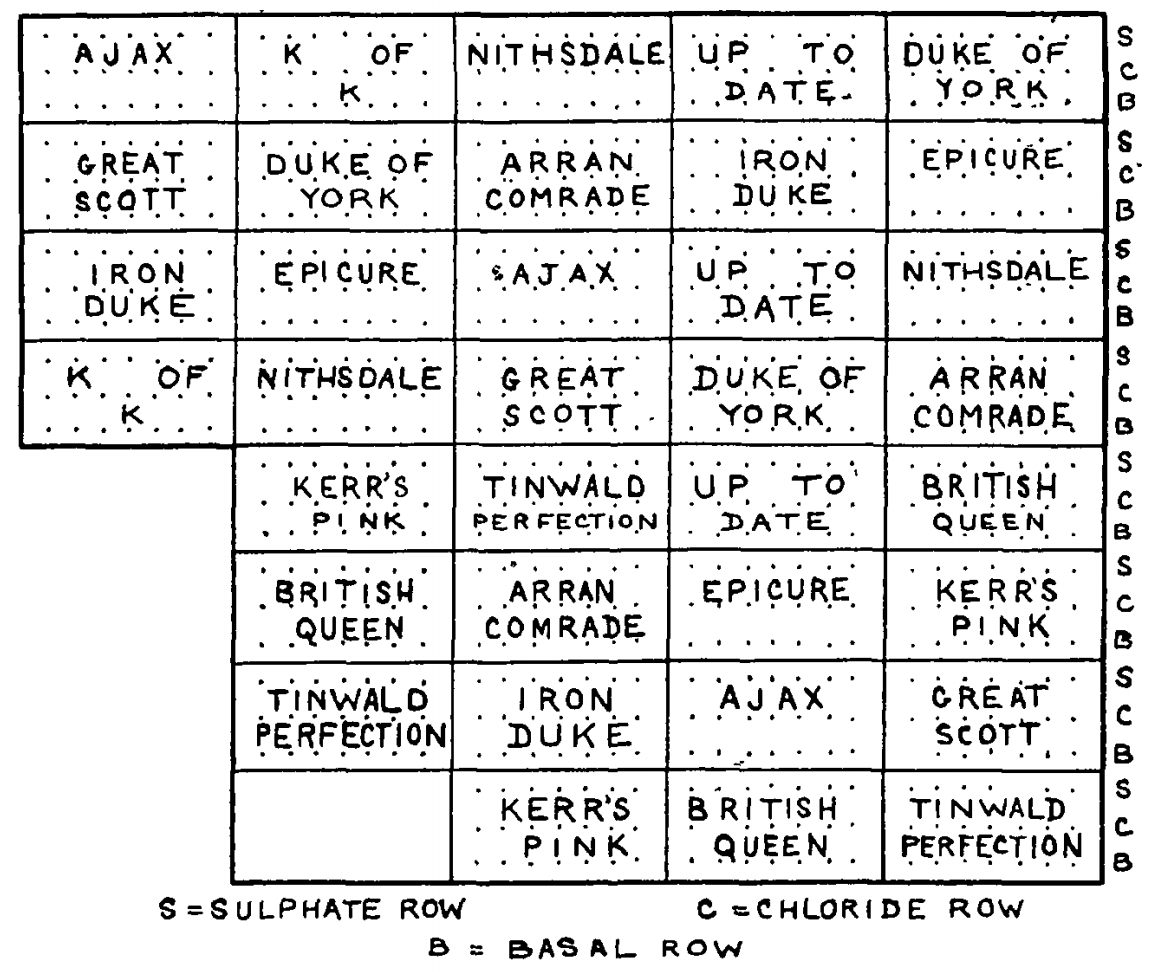
\includegraphics[width=8cm]{fisher_crop_variation.png}
\centering
\end{figure}

Fisher noted that crops will grow differently in different parts of a field due to soil and water differences.
He created two fields, one that had farmyard manure and one without.
Then each of the fields was divided into 36 plots with different potato crops at random.
Each of these rows got a different manure: sulphate, chloride or basal.
The amount of crops in pounds that was grown was recorded.
Fisher showed that the differences in the means could be compared across the fertilizers based on a decomposition of the error in terms of the various groups.

\section{Conclusion}
There is so much more to the history of statistics than this brief paper can describe.
Each man described in this essay had enormous influence and shifted how we do science as a whole.
Unfortunately many of the ideas of this time are being misused or misunderstood today such as the abuse of p-value and hypothesis testing.

\bibliographystyle{plain}
\bibliography{references}
\end{document}
